\noindent
\begin{slikaDesno}{fig/sinus_odabiranje}
    \textbf{\ID}. Континуални сигнал $x_1(t) = \sin(2\uppi f_1 t)$, учестаности $f_1 = 1\unit{MHz}$, измерен је 
    дигиталним осцилоскопом у тренуцима времена
    $t = kT_s$, где је ${T_s = 0,2\unit{\upmu s}}$, чиме је добијен дискретан сигнал $\hat x[n] = x(nT_s)$, као на слици.
    Затим је мерен простопериодични сигнал $x_2(t)$, учестности $f_2$, измерен истим поступком 
    са истом вредношћу $T_s$, чиме је добијен дискретан сигнал $\hat x_2[n] = x_2(nT_s)$. 
    Установљено је да је $\hat x_1[n] = \hat x_2[n]$. 
    На основу тог резултата, одредити могуће вредности учестаности $f_2$.
\end{slikaDesno}

\textsc{\underline{Решење}}:
Дискретни сигнал $\hat x_1[n]$, добијен од континуалног сигнала $x_1(t)$, је дат изразом 
$
\hat x_1[n] = \sin(2\uppi f_1 n T_{\rm s}) 
$. Нека је учестаност простопериодичног сигнала $x_2(t)$ записана као $f_2 = f_1 + \Delta f$, онда се за дискретан сигнал 
$\hat x_2[n]$ може писати
\begin{eqnarray}
    \hat x_2[n] = \sin(2\uppi f_2 nT_{\rm s}) = \sin(2\uppi (f_1 + \Delta f) nT_{\rm s}) 
    = \sin(2\uppi f_1 n T_{\rm s} + \underbrace{2\uppi \Delta f n T_{\rm s}}_{2\uppi k[n]}  ) \\
    = \sin(2\uppi f_1 n T_{\rm s}) = \hat x_1[n]
\end{eqnarray}
Због периодичности континуалне синусоиде, довољан је услов да је $2\uppi \Delta f n T_{\rm s} = 2\uppi k[n]$, за целобројне вредности $k[n]$.
Односно, услов да је $\Delta f = k[n]/nT_{\rm s}$. Пошто је $\Delta f$ контанта, онда мора бити $k[n] = k_0 n$, 
$k_0 \in \mathbb Z$, односно, $\Delta f = k_0/T_{\rm s}$. Закључујемо да су  могуће учестаности сигнала $x_2$
из скупа
\begin{eqnarray}
    f_2 = \left\{
    \ldots,
    f_1 - 2 f_{\rm s},
    f_1 - f_{\rm s},
    f_1,
    f_1 + f_{\rm s},
    f_1 + 2 f_{\rm s},
    \ldots
    \right\}, \qquad f_{\rm s} = \dfrac{1}{T_{\rm s}}.
\end{eqnarray}
Пошто су у конкрентом случају $f_S = 5\unit{MHz}$, то су могућа решења из скупа
$f_2\unit{MHz} \in \{\ldots, -4 ,1, 6, 11, \ldots\}$.

\begin{figure}[ht!]
    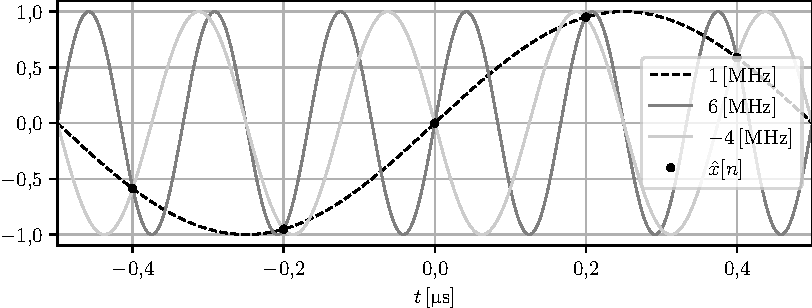
\includegraphics{fig/sinus_odabiranje_rekonstrukcija.pdf}
    \caption{Синусоиде различитих учестаности које одговарају истом дискретном низу.}
\end{figure}

Резултат овог задатка је веома важан јер наговештава проблем да је дискретизацијом 
континуалног сигнала, у општем случају, 
немогуће једнозначно реконструисати полазни сигнал. Ипак, у наставку курса, изучићемо који квалитети 
континуалног сигнала, и одабир времена $T_{\rm s}$, могу довести до једнозначне реконструкције
и много сложенијих сигнала од простопериодичног.  